\documentclass[12pt,a4paper,final]{IEEtran}

\usepackage{amsmath}
\usepackage{amsfonts}
\usepackage{amssymb}
\usepackage{graphicx}
\usepackage{verbatim}



\renewcommand{\thesubsection}{\alph{subsection}}



\title{Assignment 3\\}

\author{s316620\\}


\begin{document}
\maketitle
\newpage


\part*{Introduction}


\part*{}

\section{}

\section{Exploring the config files of the Quagga router configuration.}

\subsection{}
First configuring the Adapter1. Connect the Adapter1 to the internal network "\textit{GW\_external}"  and Adapter2 to ``\textit{GW\_SW1\_cable}''. 
When I set up the quagga interface in \textit{Assignment 2 } I removed the IP address configuration line 
\begin{verbatim}
ifconfig eth0 10.0.0.1 netmask 255.255.255.0
\end{verbatim}
from the ``\textit{/opt/booblocal.sh}''


\subsection{}
After changing the internal networks the adapters are connected to, I change the IP address assigned to each interface. This can be done using multiple ways. We can either configure it through the quagga terminal or edit the  ``\textit{/usr/local/etc/quagga/zebra.conf}'' file. 
\\	 
	 I edit the \textit{zebra.conf} file.
	Open the file ``\textit{/usr/local/etc/quagga/zebra.conf}'' and edit the IP address to the new IP address for each of the interface. 
	\begin{figure}[!h]	
	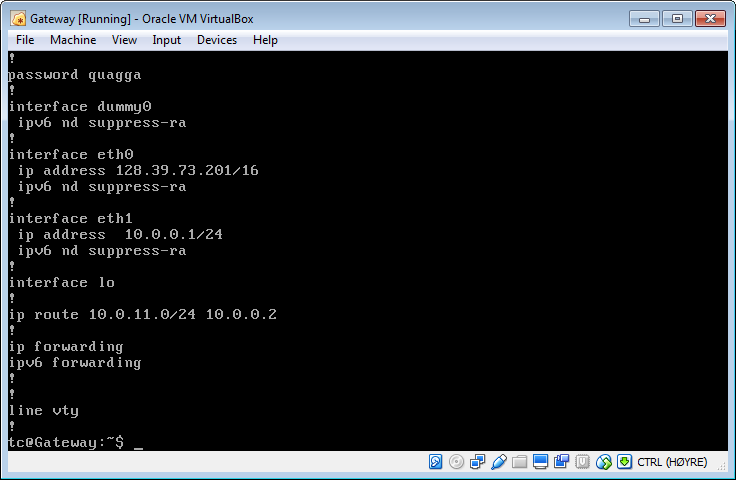
\includegraphics[width=1.0\textwidth]{2b_1.png}
	\caption{Gateway \textit{zebra.conf}}
	\label{tab:2b_Gateway_zebra} 
	\end{figure}

Save the file persistently using the \textit{filetool.sh} Then reboot. We can see that the new IP addresses are assigned to the interfaces in Figure \ref{tab:2b_Gateway_ifconfig}.

\begin{figure}[!h]
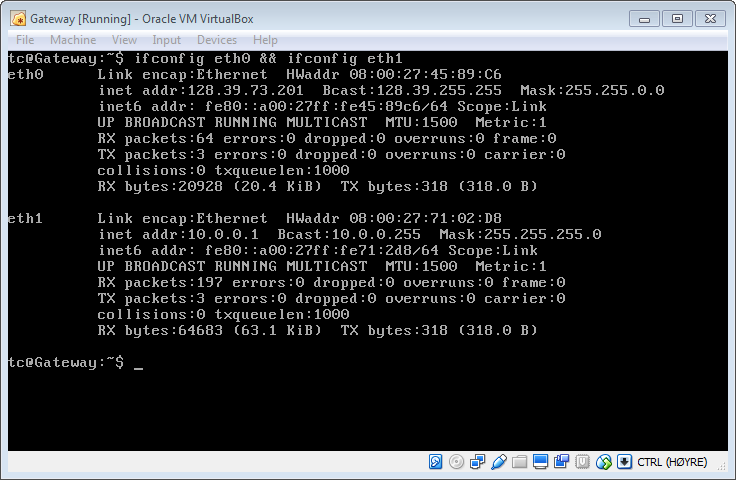
\includegraphics[width=1.0\textwidth]{2b_2.png}
\caption{Gateway \textit{ifconfig eth0 and eth1}}
\label{tab:2b_Gateway_ifconfig} 
\end{figure} 

\subsection{}
Making sure that Adapter1 (eth0) is connected to ``\textit{GW\_external}'' and Adapter2 (eth1) is connected to ``\textit{GW\_SW1\_cable}'' as seen in \ref{tab:2c_Gateway_settings}.

\begin{figure}[!h]
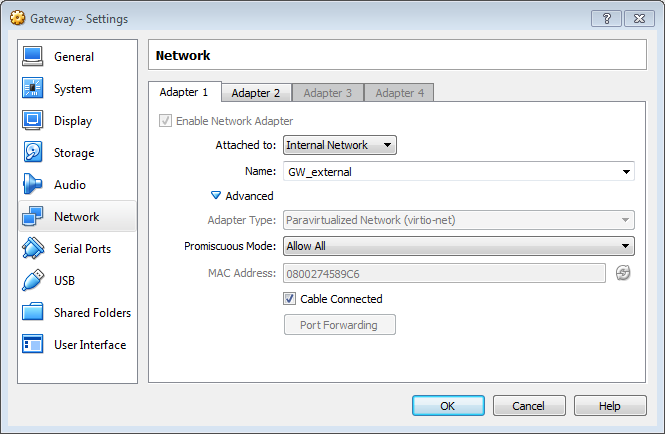
\includegraphics[width=1.0\textwidth]{2c_1.png}
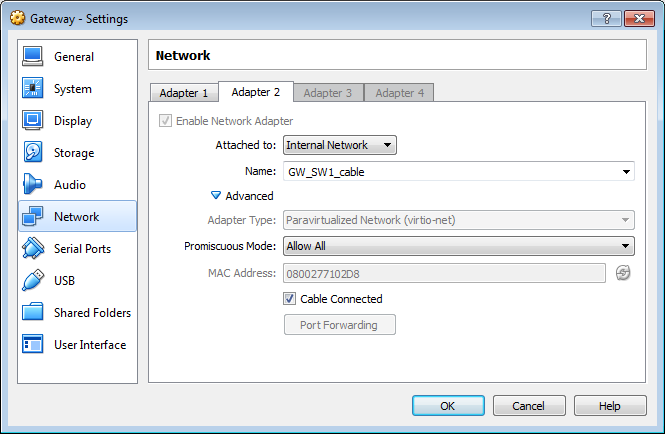
\includegraphics[width=1.0\textwidth]{2c_2.png}
\caption{Gateway Adapter1 and Adapter2 settings.}
\label{tab:2c_Gateway_settings} 
\end{figure} 

Then checking connectivity with \textit{ping} from External\_ssh to Host1 and it shows that it is connected, as seen in Figure \ref{tab:2c_xs_ping}.
\begin{figure}[!h]
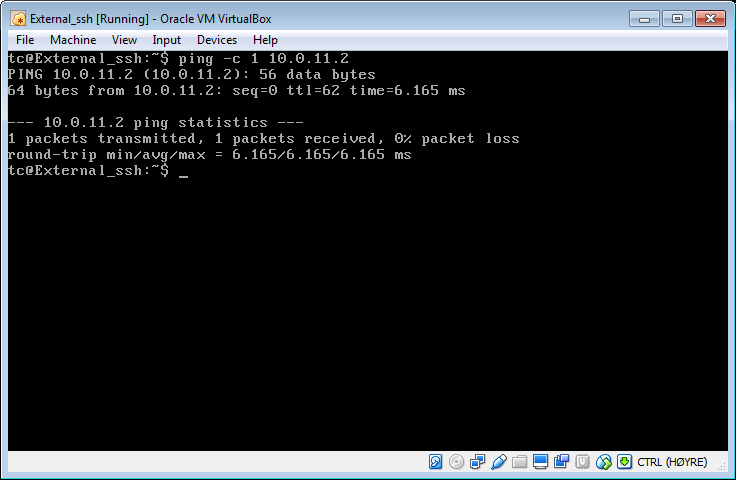
\includegraphics[width=1.0\textwidth]{2c_3.png}
\caption{Externall\_ssh \textit{ping} Host1 }
\label{tab:2c_xs_ping} 
\end{figure} 

\section{A minimal DHCP server/daemon (udhcpd)}

\subsection{}
Now I am going to install a virtual udhcp-server in the network. However, if there is a udhcp server running in the network, the udhcpc process would quickly obtain a new address from the udhcp server. This would override the manual IP address configuration that is set up. So, the udhcp process at the nodes ``Gateway'', ``Choke'' and ``Server2'' will be turned off. The udhcp-server will be ``Server2'' in this network.

The udhcp process are all turned off(\textit{killed}) in each of the nodes by running the command
\begin{verbatim}
pkill udhcp
\end{verbatim}
from the \textit{bootlocal.sh} file, before the assigning the IP addresses using the \textit{ifconfig} command. \\
\[\textit{Note: Remember to save persistently (filetool.sh) all the changes that is made.}\]


\subsection{}
Creating a persistent file ``\textit{/etc/udhcpd.conf}'' to Server2, for the configuration of DHCP-server. We get a default ``\textit{udhcpd.conf}'' file from the internet.


 \end{document}
